\chapter{Methodology}
\label{chap:meth}
\section*{Chapter Outline}
In this chapter we describe the steps taken to carry out the experiments conducted in the various experiments. We describe the tools and frameworks used to generate and process the data, and explain how these tools were used to create our own experimentation framework for the rapid simulation of a large number of uniquely generated networks.


\section{NEURON tool}
%Description the NEURON tool, how it works, and how we use it.
The NEURON tool is a simulation framework developed by researchers at Yale University for the \emph{in-silico} analysis of individual and networked neurons, and originally released in the 1990s. The framework provides a number of tools for the construction, simulation, and recording of individual cell-models from biological principle building-blocks as well as networks built from individual neuronal models. The main goal of the framework is to simulate the mathematical models that describe nerve cells, and the tools provided are intended to allow for easier interfacing with the model simulations. Use of this approach has a number of benefits over other simulation methods \cite{neuronSimEnv}. One such benefit is that the framework allows for the expression of the problem space in biological terms, without any need for the user to explicitly convert from the neuroscience-context into computational analogues. Another benefit is the supporting tools included with NEURON that allow for manipulation of the simulation environment (timesteps, type of simulation model etc.) as well as the inclusion of tools for easily collecting, converting, and graphing the measurements around the simulation space. On top of the graphing tools, the framework includes a full set of GUI-creation tools with a number of predefined "widgets", allowing for the rapid design and implementation of simulation GUIs that allow for graphical control of the simulations. Finally, the NEURON tool has had considerable work done on improving the efficiency of its backing computational engine, using "special methods that take advantage of the structure of nerve equations". The framework also has support for multi-threading which can take advantage of modern multicore processors for even more efficient computation.

\par

There are two main methods of interfacing and controlling the NEURON framework: through the High-Order Calculator (HOC) language, and through Python.\\
The HOC language was originally designed as a floating-point calculator featuring C-like syntax (and indeed was co-developed by one of the original developers of the C programming language) \cite{kernighan1979unix}. Since its introduction in 1984, the language has been extended beyond simple calculator-syntax into a more general-purpose programming language, such as through the introduction of object-oriented syntax. Its calculating background, however, makes it a suitable choice for the control of the NEURON tool due to the close relation between the neuronal cells and the mathematical models through which they are simulated.\\ %A sample section of HOC code used in the creation of these neuronal simulations is shown in listing \ref{lst:hocSample}.\\
Python support was more recently added to the NEURON framework, allowing for much the same interfacing capabilities as with HOC. As well as interfacing directly with the framework, it is also possible to interface the Python segments with HOC source files, allowing for hybrid programs to be run. The majority of the simulation code used in the course of this investigation was written in Python, with a small number of HOC-source interfaces. This allowed for the use of the large repository of Python libraries which greatly aided with the creation of the simulations and the conversion between data types. A more detailed of the specific work undertaken in interfacing with NEURON is discussed later.

\par

The basic building block of a neuronal model in NEURON is a \emph{section}. A section can be thought of as a length of cable with a specified geometry given by length and diameter. The electrical characteristic of the section is specified by the \emph{axial resistivity}, expressed in ohm-cm. Sections can be interconnected, branched, and joined to form the overall structure of the neuron. The connectivity of the sections is hierarchical in nature, in that each section has a parent section (and thus may have numerous child-sections). Each section is subdivided into a specified number of \emph{segments}. This is done for simualtion purposes, as the membrane potential is calculated at the ends of each segment within the section. As the number of segments in a given section is specifiable, the user has granular control over the complexity of the computation for each section. By defining the geometry and electrical characteristics of a neuron in term of a hierarchy of interconnecting sections, it is possible to quickly generate a computational model of the cell in the NEURON environment.
\\
Synapse models can be created in NEURON in a number of different ways. The simplest method of creating a synapse is to use one of the predefined synapse models, such as the \emph{ExpSyn} object, a construct built-in to the framework that defines a synapse with a discontinuous change in conductance at an event (i.e. a voltage spike) followed by an exponential decay. This models the concept of a release of neurotransmitters generating a resultant current in the post-synaptic dendrite, a process described previously in \ref{chap:back:neurons}. The ExpSyn object has a number of parameters that can be specified: the decay time constant ($\tau$) in ms, the reverse potential (e) in mV, and the synaptic current (i) in nA. Another more complex method of modelling synapses is to define a NEURON \emph{mechanism}, which is a mathematical description of the functionality of some process. This is quite a flexible approach as there is a greater level of control over the functionality of the process, and it is therefore possible to model specific biologic synapse forms, such as the NMDA synapse discussed in \ref{chap:back:neurons}. 
The synapse is "connected" to a section on a cell, in much the same way that sections connect to each other. At this point, a change in the membrane potential of the synapse will result in a corresponding change in the membrane potential of the section directly connected to the synapse, which can then propagate through the section and further through the entire neuronal model.
One important consideration with the form of the synapses in NEURON is that rather than respond to a potential as they would in practice, the simulated synapses instead respond to an \emph{event}. An event is a type of construct in NEURON that represents exactly that: an event. It defines a point in time in the simulation during which "something" has happened, without explicitly specifying what the "something" is. In the case of the synaptic models, the event is generally generated when the membrane potential crosses a certain threshold, indicating a voltage spike. The synapse object receives the event (without any information of the actual voltage that generated it) to which it can respond with its own event, or more commonly by adjusting its membrane potential. An event can also have a weight associated with it, which can be used to specify the intensity of the event.
\\
Another feature required for most simuations is one or more stimuli. In NEURON, a given stimulus is usually implemented in three parts: a \emph{NetStim} object, a \emph{NetCon} object, and a synapse. The NetStim object generates a spike train, similar to the type of output spike train that one might expect as the response of a neuron. This is intended to emulate some system of pre-synaptic neurons which generate a set of spikes which are delivered to the neuronal model that is to be simulated in the framework environment. The NetStim object is a built-in feature to the NEURON framework, and has the following parameters:
\begin{itemize}
    \item NetStim.interval - mean time between spikes in ms
    \item NetStim.number - average number of spikes generated
    \item NetStim.start - the desired time offset from start of simulation to generate the first spike, in ms
    \item NetStim.noise - proportion of additive noise to include, in a range of 0 to 1.
\end{itemize}
As the simulation runs, the NetStim object will generate a number of \emph{events} representing voltage spikes. These events must be delivered to a synapse of the cell being simulated in order for the cell to respond. The two objects cannot be connected in the same way as the model \emph{sections} can, as they are dealing with events rather than electrical currents. Instead, the connection is typically implemented using a \emph{NetCon} object. The NetCon object has multiple purposes, however in this case it is used to connect an event-generator (in this case a NetStim object) to an event-receiver (a synapse). No other parameter is required by the NetCon object in this use case, as it is simply delivering an event, however it is possible to also specify an event-delivery delay in ms, and an event weight.\\

Connecting 2 neuronal models together (such as in the case of the simulation of a network) is similar in principle to the creation of emulated stimuli, however instead of using a NetStim object to generate spike-events, instead a simulated neuron generates a certain output voltage over time which must be used to generate the events. This is done using a NetCon object again, however in this case it is used in a slightly different way. Previously, the NetCon object was used to simply take an event-generator and deliver the events to an event receiver; in this case, the NetCon object takes a voltage generator (i.e. the output of a neuron), and uses a pre-defined threshold on the voltage to generate a new event, which is then delivered to an event receiver. In this case, the "source" end of the NetCon is connected to the axon membrane of the pre-synaptic cell. A threshold voltage can then be specified, which represents the voltage level that the membrane must cross for an event to be generated. A delay and weight value can also be specified, as above. The output side of the NetCon can then be connected to the synapse on the dendrite of the post-synaptic cell. With this, the 2 neurons are connected and a network is formed. Artificial stimuli (such as with a NetStim) connected to the pre-synaptic cell with stimulate it, causing the neuron to generate an output voltage spike-train. This spike train is then thresholded by the NetCon object, generating events which are delivered to the synapse at the dendrite of the post-synaptic cell where the release of neurotransmitters is simulated, raising the potential of the section. This is the functionality of the neuronal simulation which were used in this study. In practice, multiple stimuli are used, and multiple NetCon->synapse connections are used between cells in the network with varying delay, threshold, and weight parameters.\\

With the network of neurons created and under simulation, it is necessary to also measure the voltage at various points amongst the neurons. This measurement is implemented using a NEURON \emph{Vector}, another built-in object in the framework. The Vector object is similar to the C++ std::vector class, representing a dynamic array that can be added to during runtime. In the NEURON framework, the Vector object represents a list of floating-point values and can be programatically added to and read from. An addition function of the Vector object comes from the use of its member function \emph{Vector.record()}. This function allows the user to specify a section voltage-reference (a member of each NEURON section representing the membrane potential of the given section), and it will then record the section voltage during simulation. The user has additional parameters to specify either the recording time-step (the discrete steps in time at which the voltage will be sampled), or even a predefined vector of time-points to sample at. Following simulation, the Vector object will contain the recordings of the section which can be easily converted to Python-native lists for manipulation, or saved to disk (or indeed both).\\

\subsection{Cell-data Source}
%Blue-brain project and the model files they provide. What the files contain, and how they're used in NEURON
In \ref{chap:relwork:bbpData} we discussed the data collected and supplied by the Blue Brain Project (BBP). This data is supplied in a format that is compatible with the NEURON framework, including sample HOC files for initiating and simulating single-cell networks. Each cell supplied is categorised by the layer, m-type, e-type, and variation (multiple variants may exist for the same layer;m-type;e-type group). For example, the cell titled "L1\_DAC\_bNAC219\_1" represents a layer 1 cell of DAC m-type and bNAC e-type. For each cell, a number of data-files are supplied. One of the main files is the morphology descriptor. This file contains the complete description of the entire morphology of the cell, formatted as the NEURON-compatible section-segment hierarchy. Rather than manually specifying each section in HOC code, the morphology descriptor can be loaded in about 3 lines of code using the \emph{Import3d\_Neurolucida3()} and \emph{Import3d\_GUI()} functions. These functions read the section descriptor file, and construct the entire cell morphology in the environment. The morphology is also pre-segregated by cell-portion (soma, dendrites, axon etc.) and each can be explicitly accessed. The supplied data also includes a programatic of the cell's biophysical properties. These properties represent the specific electrical characteristics of various sections within the neuron and are vital to accurate simulation of the cell. The characteristics are defined by NEURON mechanisms, discussed previously, which represent the response of an object to some stimulation in a mathematical sense. A description of the cell's synapses are also included. This includes the location, synapse type, and synapse parameters for each synapse in the dendritic branches of the cell, which are again easily loaded programatically. \\
\begin{figure}[ht]
    \centering
    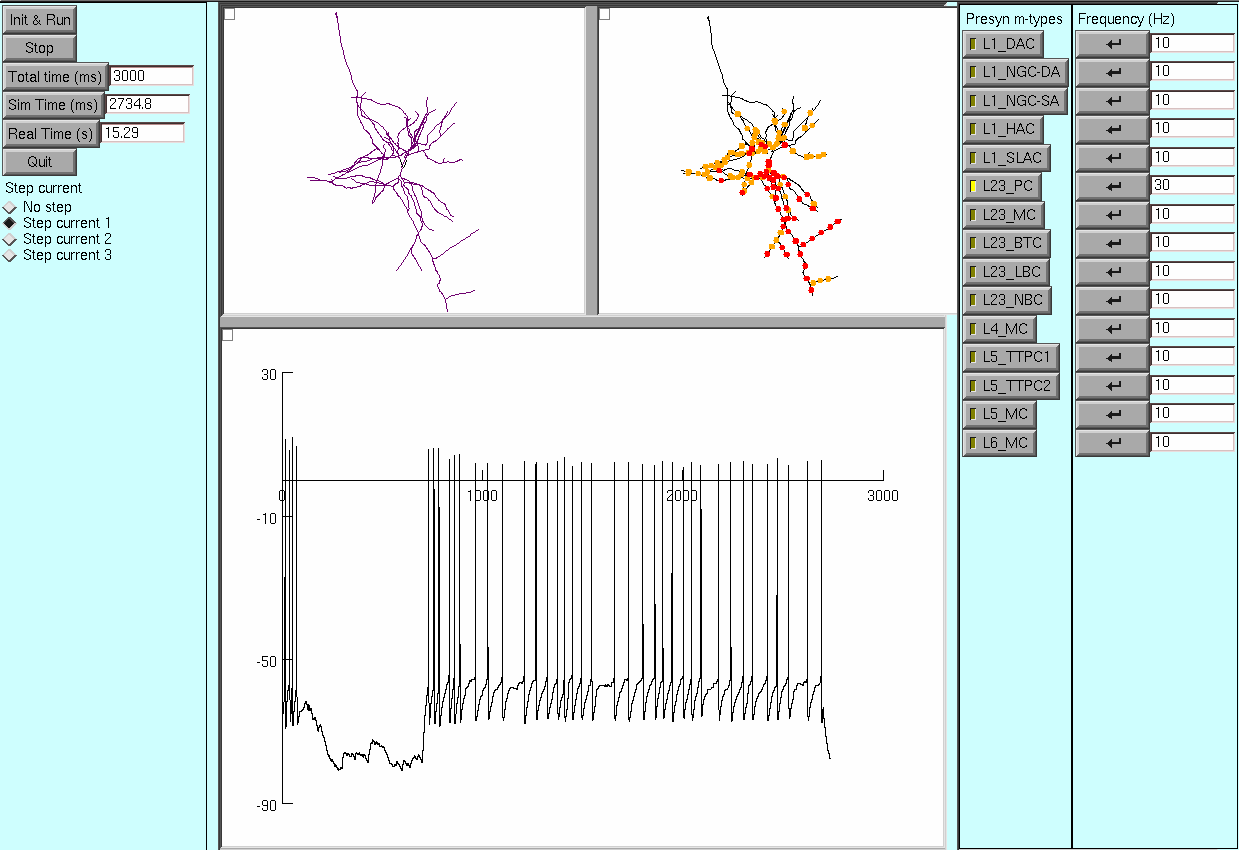
\includegraphics[width=0.8\textwidth]{04-Methodology/nrnSample.png}
    \caption{NEURON simulation GUI generated by BBP data files}
    \label{fig:bbpNrnGui}
\end{figure}

Along with the various cell descriptors, sample HOC files are also included which instantiate a NEURON session, load all of the cell data into the session, sets up a number of pre-synaptic stimuli (using the NetStim approach discussed above) and then constructs a GUI interface for interactively controlling the simulation. The result of running this sample HOC instantiation file is shown in Figure \ref{fig:bbpNrnGui}. The left-hand panel of the generated GUI are used to control the simulation, allowing the user to start and stop the simulation along with specifying the length of the simulation to run. The centre-top panels show the loaded cell's morphology and areas on the cell to which synapses are connected and stimulated. The lower panel shows the graph of the membrane voltage over time (updated in real-time as the simulation runs), which clearly shows the spike-train output of this neuron. The right-hand panel is used to enable/disable the various pre-synaptic emulated cells (using NetStim objects) that can be connected to the neuron in the simulation. The frequency of the spikes (i.e. the interval property of the NetStim object) can also be specified to select the stimulus intensity.



\subsection{Python Backend and Support Library}
%Description of the NEURON Python API and how we used it to create the Neurpy library for quickly analysing cortical circuits.\\
%Layout of the software, output formats etc.

While the sample files given by the BBP are extremely useful and informative, they are limited in that it is not inherently easy to connect multiple cells together to form a multi-cellular network. As well as this, the use of the GUI is not a scalable approach when generating a large set of training data. For this reason, we developed a Python library to address these issues \cite{neurpyGit}.\\
The library, referred to as \emph{Neurpy} uses the NEURON-Python API to more easily construct simulations of any network form, while also allowing for either GUI interfacing (for interactive/debug purposes) as well as a more lightweight "headless" interface where the simulations are run entirely though the Python code without any need for user interaction. This headless approach also allows us to easily run multiple simulations in parallel, taking advantage of modern multi-core CPUs to accelerate the generation of test data.\\
Neurpy makes use of the data supplied by the BBP to construct the simulations. For simulation, a Neurpy "Environment" object, \emph{NeurpyEnviron}, is set up, which represents a NEURON session including all cells in the environment space, stimuli, recording vectors etc. and exists for the duration of the simulation. The \emph{pyCell} class was defined to represent a single BBP-supplied cell. The class loads in all relevant data from the cell dataset, such as the morphology, biophysics, and synapses, and allows for easy manipulation of the cell as a single, addressable unit in the environment. The cell can be translated to different points in space, however the main benefit of this class is the hierarchical structure of interconnected cells. By calling the \emph{pyCell.addChild()} function and passing another cell as a parameter, the Neurpy library will automatically connect the parent cell to the child cell using a number of NetCon->Synapse connections as described previously. Through the parameters to this function, the number of synaptic connections, as well as the delay and weight for the connections can be specified.\\
The Neurpy library also allows for easier creation of network stimuli and membrane potential measurements (referred to as \emph{probes}). Network stimuli are provided by the \emph{CellStim} class. This class represents a NetStim->NetCon pair and can be connected to one or more synapses on a given pyCell object. Another feature of the CellStim class is the probabilistic amplitude-keying option. By supplying a "symbol probability" the CellStim object will automatically enable and disable itself as the simulation run. This is to simulate the transmission of "symbols" as defined for the information theory equations in Section \ref{chap:back:infTheory}. The object keeps a list of the toggle-states it was in throughout the simulation which can later be used in processing to estimate the mutual information of the synaptic link (discussed in more detail later). The network probes (membrane measurements) were not implemented in a specific class as the creation of the probes is quite simple, requiring only the creation of a Vector object, and the linking of that Vector to a cell section. The Neurpy library does this and connects the Vector to the soma of a specified cell, adding the Vector object to a global list.\\
At this point the network is created as the individual cells are loaded and interconnected, the stimuli have been generated and connected to the cell models, and probes have been set up to record the network as the simulation runs. At this point, there are two options available to the user: create a GUI window for interactive simulation, or run a headless simulation. In the first case, a GUI of the same structure as Figure \ref{fig:bbpNrnGui} is created with all loaded neurons visible in the centre-top panels. The user can then set simulation parameters and run the simulation, observing the recorded voltage in the graph panel. This does not produce any simulation data that is saved to disk, and so was generally only used for debugging purposes. The second case (headless simulation) is done through calling the \emph{NeuronEnviron.runSimulation()} function on the Neurpy environment object, passing the filepath of the desired output data. The Neurpy library then calls on the NEURON framework to begin simulating the objects in the current session. After the simulation has completed, the library collects all the Vector recordings that had been specified, converts them to a native Python format, concatenates all the voltage data-points and exporting as a comma-separated value (CSV) file, saved to the specified data path. This entire process can be seen in listing \ref{lst:sampleNrpyCode}. In this code snippet, the Neurpy library is first imported, and an environment session is started by calling \emph{NeuronEnviron}. The environment requires the location of the BBP model and mechanism data as parameters, such that the relevant data can be loaded when creating cells. Next, 2 different cells are created: \emph{cellA} is from layer 6, with m-type BP and e-type bAC, while \emph{cellB} is from layer 1 with m-type DAC and e-type bNAC. Following this, \emph{cellB} is translated in space by 100 $\mu m$ in the y-direction. We then add \emph{cellB} as a child of \emph{cellA}, specifying that the synapse should be excitatory ("true" for excitatory, "false" for inhibitory), and that 6 synapses with weight 1.0 and delay 1.0ms should be used to connect the two cells. At this point, the 2-cell network has been created, so we can either generate the GUI for interactive simulation (as in the first branch of the if-statement) or we can run a headless simulation, passing a local filepath as our desired output file. At the end of the simulation, all output measurements will be saved to "simData.csv" and the script will exit, destroying the Neurpy (and thus NEURON) environment and freeing up memory before exiting.\\ 



While this method of hard-coding networks in Neurpy is viable and certainly easier than with the given HOC source files in the supplied BBP data, it is not ideal for the automatic simulation of large sets of networks which is required by this investigation. For this reason, a network-descriptor feature was added to the Neurpy library whereby the NeuronEnviron object can load in a description of a simulation network (including all cells, cell-to-cell connections, stimuli, and probes), which it can then automatically construct in the given session and simulate. This allows for easier scripting of the experimental process, allowing for the generation of large sets of data.



\subsection{Network Descriptor}
For the specification of networks, an XML-based descriptor was defined, similar in concept to the \emph{GraphML} format for describing network graphs. XML (eXtensible Markup Language) is a type of markup language which, similar to JSON, allows for the hierarchical description of a set of parent-child relations, specifying key-value parameters for each entry. The base block of an XML document is an \emph{element} which is a named block with a set of key-value parameters, as well as 0 or more sub-elements. There is no inherent constraint on the naming of the elements or the parameters, as the functionality is based entirely on the interpretation of the document. A simple example of an XML document is shown in listing \ref{lst:sampleXml}. The first line in this listing is the document's metadata, and contains information about the format of the rest of the document. After this, an element of type "node" is created with an ID parameter of 0, and another parameter of value 120. The node element also has 2 children, one is another element of type "node", and the other is an element of type "testData". Neither of these elements have further child elements, and so can be terminated using the "/>" terminator. The termination of the parent element can be expressed using "</node>" after all of its children have been specified.
\begin{lstlisting}[language=XML,label=lst:sampleXml]
<?xml version="1.0" encoding="UTF-8"?>
<node id="0" some_param="120">
    <node id="0_0" another_param="1" />
    <testData/>
</node>
\end{lstlisting}
As the naming of the XML elements and parameters is entirely implementation dependent, we can therefore define our own XML-based descriptor to describe the networks that we will be simulating:
\begin{enumerate}
    \item The base element of the hierarchy is an element of type "Neurtwork". All network elements will be some child/grandchild etc. of this base element.
    \item Individual cells are specified by an element of type "cell" with parameters:
    \begin{itemize}
        \item cellType - a string representing the corresponding cell in the BBP dataset
        \item id - a session-unique ID for the cell in the environment
        \item label - an optional label string for the cell
    \end{itemize}
    \item All individual "cell" elements are direct children of a single "cells" element
    
    \item Cell-to-cell connections are specified by an element of type "edge" with parameters:
    \begin{itemize}
        \item id - a session-unique ID for the edge in the environment
        \item source - the ID of the source cell
        \item target - the ID of the target cell
        \item connCount - the number of synaptic connections in the edge
        \item connType - the synapse type: 1 for inhibitory, 0 for excitatory
        \item delay - the delay in ms of the edge
        \item weight - the weight of the edge
        \item label - an optional label string for the edge
    \end{itemize}
    \item All individual "edge" elements are direct children of a single "edges" element
    
    \item Stimuli are specified by an element of type "stim" with parameters:
    \begin{itemize}
        \item id - a session-unique ID for the stimulus in the environment
        \item target - the ID of the target cell
        \item delay - the delay in ms of the stimulus connection
        \item prob - the symbol-probability of the stimulus
        \item label - an optional label string for the stimulus
    \end{itemize}
    \item All individual "stim" elements are direct children of a single "stimuli" element
    
    \item Measurement probes are specified by an element of type "probe" with parameters:
    \begin{itemize}
        \item id - a session-unique ID for the probe in the environment
        \item target - the ID of the target cell
        \item tag - an optional label string for the probe
    \end{itemize}
    \item All individual "probe" elements are direct children of a single "probes" element
\end{enumerate}

An example of a network specified with the above format is shown in listing \ref{lst:sampleNetXML}. This network consists of 2 cells, a layer 1 DAC m-type and bNAC e-type cell and a layer 1 NGC-SA m-type and cNAC e-type cell. The first cell connects to the second through 5 excitatory synapses with a delay of 5ms and a weight of 2. A single stimulus is connected to the first cell, with unspecified probability (disables the symbol-probability keying). Finally, 2 probes are specified, one for each of the cells. The tags specified in the network are used as column-headers in the output data file for easily distinguishing between the membrane voltages of the two cells.


An extension was made to the Neurpy library to accommodate the XML-based network descriptors. This extension was defined in a class called \emph{Neurtwork} which takes a path to an XML network descriptor file, reads and decodes the various elements in the document, and constructs the network in a given Neurpy session. The network loading is done entirely automatically from the XML description, and requires no further user input. Prior to simulation, however, the user may modify the session, such as through the translation of some cells (which can be addressed by their XML-defined ID parameter).\\
The benefit to this approach is that the running of the simulation can become more automated. For example, given a folder of individual network description XMLs, the code in listing \ref{lst:sampleNetRun} can be used to run through an arbitrary number of simulations (limited only by the number of network descriptors), constructing the network, running the simulation, and saving the output measurements to a separate folder. As well as this, the number of network descriptors could easily be subdivided and allocated to be run on separate CPU cores, which again allows for a speed-up in simulation time.
\begin{lstlisting}[language=Python,label=lst:sampleNetRun]
import neurpy, os
validFiles = os.listdir( "./networks" )
for idx, netXml in enumerate( validFiles ):
    neurEnv = neurpy.NeuronEnviron( './modelBase',
                                    './modelBase/globalMech' )
    neurEnv.loadTopology( netXml )
    neurEnv.simulate( "./output/v_data%i.csv" % idx )
\end{lstlisting}


% With the network represented in NEURON, a number of simulations were run. The soma membrane potential was measured for each of the cells, and a plot with the L1 and L6 measurements is shown in figure \ref{fig:sm_l1-6}. This figure illustrates the effect of signal propagation with multiple paths to end-nodes, where a single spike in the L1 cell often results in 2 spikes in L6 as the impulse from L1 arriving at L6 twice, with a delay between the arrivals due to different propagation times along the respective paths. One factor that can be attributed to the difference between the observed spike trains of the L1 and L6 cells is the biophysical properties of the cell itself\cite{markram2015reconstruction}, as well as the properties of the link between the neurons.\\
% With the reference network above completed, work was started on creating a Python framework which will support simplified construction and simulation of various network topologies in a consistent and scriptable manner. Using Python as the frontend language has a number of benefits over the HOC language used for the first example, namely that there is much better support for third-party libraries which may be helpful in future for handling intricacies such as complex network tracking.\\
% The basis for this Python framework is the creation of a library dubbed \emph{Neurpy}\cite{Neurpy}. This library serves as an interface between a Python script and the NEURON backend, dealing with the boilerplate code of any program using NEURON, such as context creation, cell morphology/mechanism loading, network construction, GUI creation, and running the simulation/collecting measured data. In this way, the frontend script for the creation and simulation of a simple 2-cell network takes the current form:
% \begin{lstlisting}[language=Python]
% import neurpy
% neurEn = neurpy.NeuronEnviron( './modelBase',   # Base directory of cell data
%                               './modelBase/globalMech' ) # Mechanism directory
% cellA = neurEn.createCell( 'L6_BP_bAC217_1',    # Name of cell directory
%                           'bAC217_L6_BP_b41e8e0c23' ) # Name of cell
% cellB = neurEn.createCell( 'L1_DAC_bNA219_1', 
%                           'bNAC219_L1_DAC_ec2fc5f0de' )
% cellB.translate( [ 0.0, 100.0, 0.0 ] )
% cellA.addChild( cellB, 0.6 )    # Connect cellA to cellB
% if genGui:
%     neurEn.generateGUI().createMainWindow()
% else:
%     somaMeasurements = neurEn.simulate()
% \end{lstlisting}
% As can be seen, the library supports both creating a GUI instance (for displaying real-time information and visualising the network structure) as well as running the network simulation without any visual frontend (for scripting and generating banks of test data).

\section{Network Generation}

While the ability to load in XML-based network descriptors makes it easier to construct session-by-session networks to be simulated, it still requires the networks to be hand-written. Thankfully, the statistical data provided by the BBP can be used to automatically generate unique networks that fit within their supplied distributions, exporting the network in the predefined XML format that can be loaded and simulated in Neurpy. As discussed in \ref{chap:relwork:bbpData}, the BBP provided a number of useful metrics on the pathway data between connecting cells. Using this data, a network generator script named \emph{NeurGen} was constructed in Python. \\
NeurGen functions by loading the JSON-formatted statistical data on the physiology and anatomy of each cellular pathway, building an internal database of statistical distributions for each of the connective parameters, and then generating a semi-random network that is unique in layout, yet still fits to the given distributions. In other words, if one were to generate a large number of these "random" networks and then recalculate the distributions for the same connective parameters, the end results should be close to the distributions given by the BBP. This means that the generator will create anatomically correct networks that would be expected to be found within the neocortex.\\
One method of creating networks using NeurGen is through the \emph{createRandomNetwork()} function. By passing the number of cells that should be in the network to the function, it will create and return the randomly generated network. The generated network has no complex/branching connections, it is a serial line of neurons with a single path from the head cell to the tail cell. The network is generated iteratively; the first cell is selected at random from the set of all possible cells. With the head cell selected, it is temporarily named the pre-synaptic cell. The generator then finds all pathways from the statistical data that has this cell as a pre-synaptic type. With the list of possibly pathways found, a probabilistic score is assigned and the network selects the pathway from the set based on the "connection probability" parameter in the pathway anatomy. With the pathway selected, so too is the post-synaptic cell. Other pathway parameters can then be taken (such as the distribution of synapse-count per connection, edge delay, etc.) and the Python function \emph{normal()} is used to sample the distribution. The \emph{normal()} function takes a given value for the mean and standard deviation of a distribution, and samples it. With the connection between the two cells set up, the generator can now temporarily treat the post-synaptic cell as the new pre-synaptic cell, and repeat the process. This is repeated until the required number of cells have been found.\\
With the cells selected, the generator then assigns a stimulus to the head cell. As well as this, probes are assigned to each of the network's cells. At this point, the network is fully defined and it can be returned to the caller where it can then be written to the disk as an XML-formatted file. Using this network generator, we can generate a large amount of sample networks in a very short amount of time and with minimal effort. A snippet of code using the network generator to create 10,000 unique networks with between 5 and 20 cells per network is shown in listing \ref{lst:netGenSamp}.
With the networks generated, the directory containing the descriptors can then be used in the form of the code snippet in listing \ref{lst:sampleNetRun} to simulate all networks automatically.

\subsection{Template to Topology Generation}
The generation of random networks can be useful in some circumstances, however for this investigation we deal with specific network topologies that cannot be constructed through the \emph{createRandomNetwork()} function described above. For this reason, the NeurGen tool was extended to accept as input a topology template. The template takes a form quite similar to the XML-network descriptor used by Neurpy, however the major difference is that it keeps only the overall network shape (number of cells, which cells connect where, the stimuli, and the probes) without requiring any specific data to be specified about any of the network components. Cell types requirements can be specified using a regular expression (a method used for matching against strings) where the user may specify an expression that a cell must match in order to be selected for that node. In this way, the network shape can be maintained, while the cell-types that slot into the topology can be randomly selected from a user-constrained set. An example network template for a 4-leaf star topology is shown in listing \ref{lst:4leafTop}. Here we can see that the central node of the star may only be a layer 1, m-type DAC, e-type bNAC cell. Meanwhile, "Node1" of the network must be from layer 2, with no constraint on m-type or e-type. The final 3 star nodes are not constrained at all and can be any cell, provided the pathway data exists for it.\\
By running the NeurGen \emph{createNetwork()} function and passing the filepath of this topology template, the generator will again create a network that fits both to the statistical distributions given by the BBP as well as to whatever cell-matching constraints listed in the template file. In this way, an arbitrary number of unique networks of a specific topology may be generated and simulated, offering a wide variety of simulation data for analysis.

\section{Simulation Framework}
\begin{figure}[ht]
    \centering
    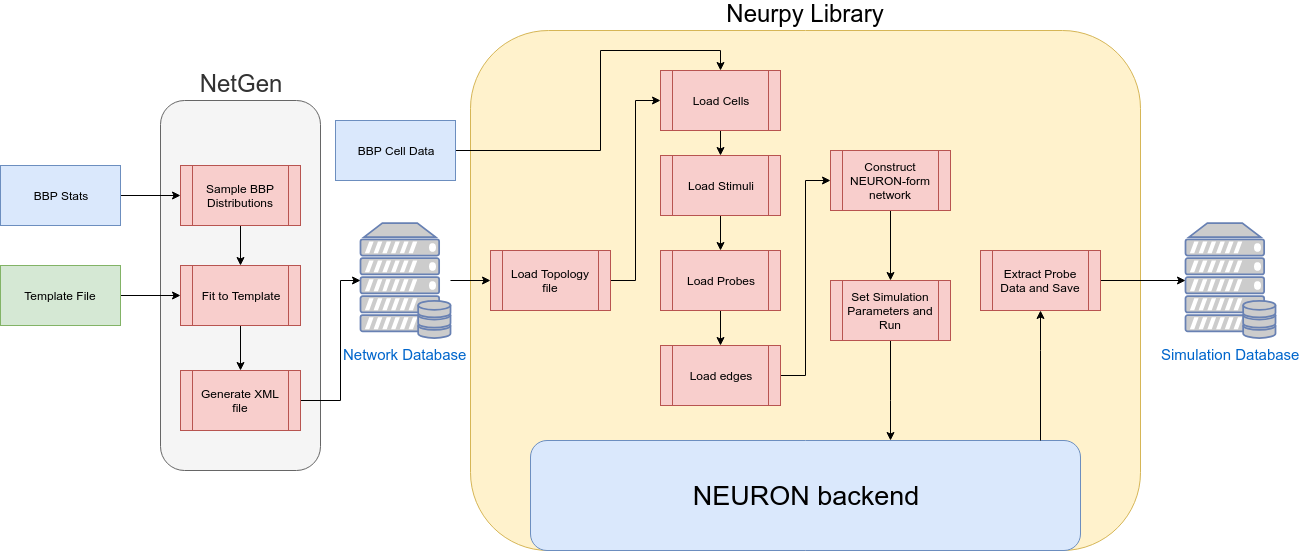
\includegraphics[width=\textwidth]{04-Methodology/SimFW.png}
    \caption{Structure of experimental environment}
    \label{fig:nrpySimFw}
\end{figure}
At this point, all the components of the simulation framework have been defined. An overview of the entire process is shown in Figure \ref{fig:nrpySimFw}. The general flow of this process is from left to right. On the left we begin with the network generator. We feed the statistical data on the cell-to-cell pathways from the BBP along with a topology template into NeurGen. Within NeurGen we can then generate a large number of unique individual networks, which we store as the "Network Database". After the database of networks has been created, we can begin feeding this into the Neurpy library, file by file. For each network file, Neurpy loads the specified cell model data from the BBP, loads and connects the required stimuli, loads and connects the required measuring probes, and finally connects the cells together to form the in-session network. Following this, the session simulation parameters are set (timestep, simulation length etc.) and Neurpy instructs the NEURON backend to begin the simulation. After the simulation has completed, all data is extracted from the probe vectors, converted and concatenated in a Python-native format, before being written to the disk. By repeating this for all network files, we create the "Simulation Database" which contains the voltage-vs-time data for each probe in each simulation, which we can then use for analysis.\\
A complete listing of the code used to run the simulations from the network files is shown in Listing \ref{ap:simCode}. This is the code that was run over the course of several days to simulate over 100,000 individual networks, and so it was made to use multiple cores to accelerate the simulations. When running, each process reports its current network ID (an index within the list of overall networks), as well as its current timestep in the simulation. The code also calculates the average number of simulations per minute to help estimate the amount of time remaining in the simulation of the network set.

\section{Investigation of Neuronal-Link Parameters}
\subsection{Simulation Dataset}
\label{chap:meth:llMeth}
%TODO: Description of the network topologies used to generate the dataset; basically just random 2-cell networks with varying levels of synaptic connections, distance, cell types etc.

The cortical networks for the study of the link-level parameters between the neuronal cells were generated using the NeurGen script described above. A simple 2-cell topology template was passed to the generator which defined a network of 2 cells (with no constraint on cell type), a stimulus on the "head" node, and a probe on each node. As this portion of the investigation deals with the link-level parameters between any 2 cells in the cortical circuits, there was no need for a topology more complex than 2 cells. The simulator script was then modified slightly so that after the loading of each topology (but prior to the running of the simulation) some parameters of the link were forcibly varied. These parameters included the link delay and weight, the distance between the nodes, as well as the interval, delay, weight, and symbol probability of the stimulus. These variations were output to a separate "metadata" file for each simulation such that they could be used in the analysis to find correlations in the data. After this, the network was simulated with a simulation length of 1000ms.

\subsection{Train Discretisation and Probability Analysis}
% Explanation of the process for discretising the voltage-time spike trains into a binary series, and the associated probability analysis to get uncertainty and mutual information.
The first step in the probabilistic analysis is to discretise the voltage-time spike trains into a binary series, similar to the process followed in \cite{spikeTrainInfo} as previously discussed in Section \ref{chap:relWork:nrnLinkParams}. In our case, the process undertaken was as follows:
\begin{enumerate}
    \item Threshold the spike-train - values above $V_{thr}$ are set to 1, all other values set to 0
    \item Subdivide the thresholded train into a number of windows of length $L_{w}$
    \item Check for the presence of a spike within the window, set the window-value to 1 if found, 0 otherwise
    \item Convert the window-interval values into a binary sequence
\end{enumerate}
This process is shown graphically in Figure \ref{fig:discrTrain}. Here, the "discretise voltages" plot represents the thresholded spikes, and the "discretise time" plot represents the subdivision into windows.

\begin{figure}[ht]
    \centering
    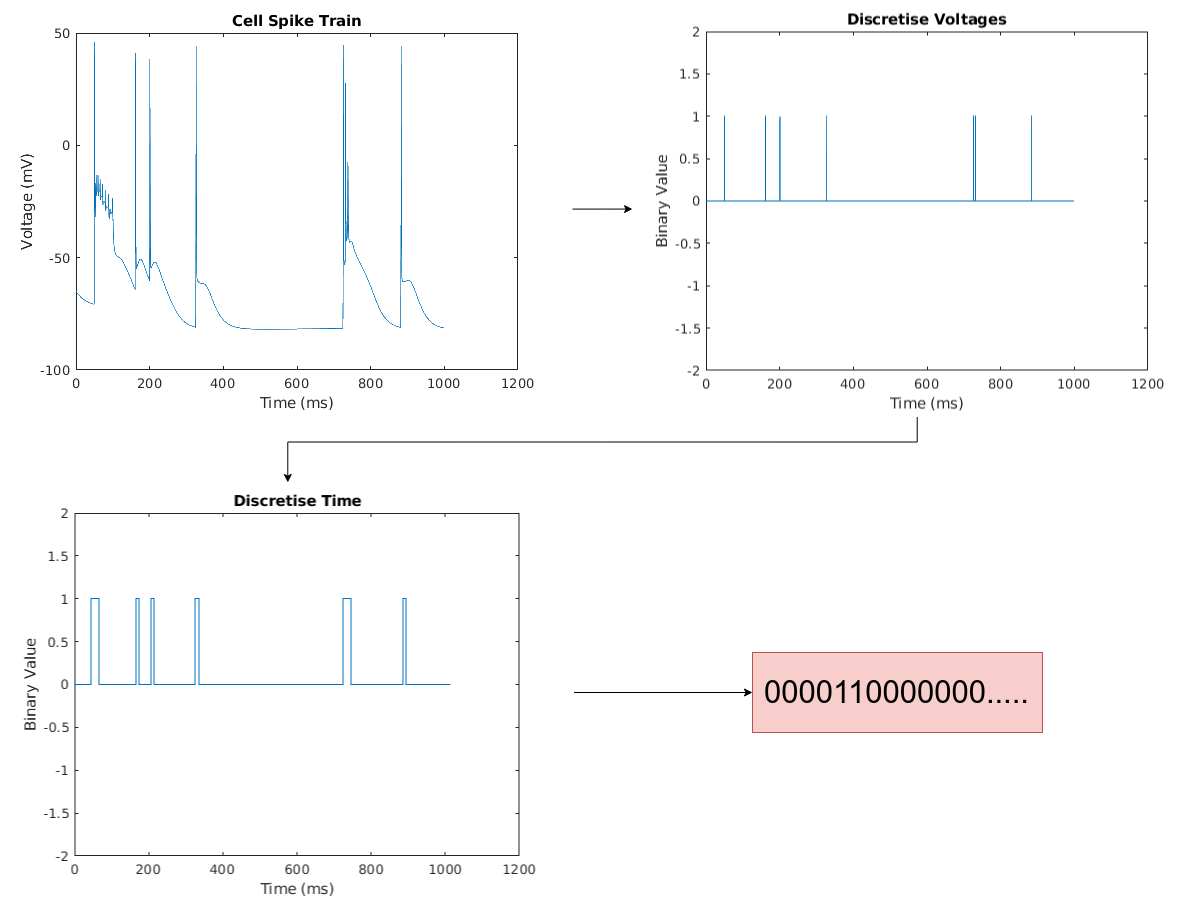
\includegraphics[width=\textwidth]{04-Methodology/descrTrain.png}
    \caption{Process of spike-train discretisation}
    \label{fig:discrTrain}
\end{figure}
The binary output sequence of this process represents the symbol of the system; in this case our symbol is 1 bit and so our symbol set can be described as $S=\{s_{1}=0, s_{2}=1\}$. Here we can calculate the binary sequence from the head cell (which we can represent as a random variable $X$) as well as from the tail-cell (represented as random variable $Y$) With this in mind, we can use the equations described in Section \ref{chap:back:infTheory}, specifically equations \ref{eq:entropyDiscr} and \ref{eq:mutualInf} to calculate the entropy of the head-cell and mutual information of the cortical link. The probability mass function (PMF) of both X and Y (that is, $P(X)$ and $P(Y)$) can be calculated from their respective binary sequences. We can then apply various forms of Baye's rule, along with further analysis of the two binary sequences, to obtain the joint PMF ($P(X,Y)$) and the conditional PMF ($P(X|Y)$) for use in the calculation of the mutual information of the cortical link.

\subsection{Delay Estimation}
For the estimation of the cortical link, we employ a simple cross-correlation analysis. The cross-correlation function describes the relation between two signals across a series of time shifts, and is described by
\begin{equation}
    \label{eq:xcorr}
    r_{xy}(l) = \sum_{n=-L}^{L-1}x(n)y(n-l)
\end{equation}
where $r_{xy}$ is the cross-correlation of $x$ and $y$ and L is the number of lags (time shifts) to calculate for in the positive and negative direction. Conceptually, a spike in the head cell should result in a spike in the tail-cell separated roughly by the delay as the spike crosses the synaptic connection. As a result, we should find a peak in the cross-correlation between the voltage measurements of the two cells as the time shift approaches the delay since at this time-shift the signals should be relatively well correlated.\\
While this approach is quite basic and may not be overly accurate, it is a first step in expressing the characteristic function of the delay in the neuronal link, which is an important concept when applying network tomography to estimate link-level delay \cite{netTomFour},

\section{Cell Classification}
\subsection{Feature Extraction and LNP Estimation}
% TODO:Explanation of the process followed to estimate the LNP filter coefficients to a specified order, and other methods that this could be implemented (i.e. iterative rather than analytical).\\
% Discussion of other features that could be used.
As previously mentioned, the Linear-Nonlinear-Poisson (LNP) cascade model can be used to model and characterise the response of a neural cell. Generally, this is computed using the spike-triggered-average (STA) of the stimulus sequence \cite{lnpInBrain} however this approach is more appropriate when dealing with external stimuli such as a spatio-temporal screen.\\
For this reason, another approach was taken to estimate some of the parameters of the LNP model. As we are not intending to recreate the spike train of the neuron, we can disregard the Poisson-spike generation portion of the model. As well as this, in the interest of simplicity, we will disregard the nonlinear component as the linear component should have a higher proportion of the overall characterisation.\\
The problem in this case is then to calculate the linear filter that best represents the response of the cell, to a predefined number of filter coefficients. This is referred to as \emph{System Identification} \cite{sysIdA}\cite{sysIdB}. The theoretical principle here is: given the linear system 
\begin{equation}
    \label{eq:firLinSys}
    y = x \star h
\end{equation}
estimate the value of $h$ to a limited order that best produces the output sequence $y$ from input sequence $x$. If we take this to be representative of a finite-impulse response (FIR) filter, we can describe the system as

\[
\begin{bmatrix}
    y_{0} \\
    y_{1} \\
    y_{2} \\
    y_{3} \\
    \vdots \\
\end{bmatrix}
=
\begin{bmatrix}
    x_{0} &    0  &    0 &     0  &    0 \\
    x_{1} & x_{0} &    0 &     0  &    0 \\
    x_{2} & x_{1} & x_{0} &    0  &    0 \\
    x_{3} & x_{2} & x_{1} & x_{0} &    0 \\
    \vdots & \vdots & \vdots & \vdots & \vdots \\
\end{bmatrix}
\begin{bmatrix}
    h_{0} \\
    h_{1} \\
    h_{2} \\
    h_{3} \\
    h_{4} \\
\end{bmatrix}
\]
for a sample 5-order filter \cite{sysIdC}. This system is not invertible to solve for $\vec{h}$ as $\boldsymbol{X}$ is not square, it is possible to solve for $h$ under "general conditions" through the use of the \emph{pseudoinverse} of $\boldsymbol{X}$. This can be more specifically defined by the Moore-Penrose pseudoinverse of $\boldsymbol{X}$, so $\vec{h}$ is given by
\begin{equation}
    \label{eq:estFilter}
    \vec{h} = (\boldsymbol{X}^{T}\boldsymbol{X})^{-1}\boldsymbol{X}^{T}\vec{y}
\end{equation}
where $\vec{h}$ is the estimated filter, $\boldsymbol{X}$ is the equivalent time-delayed input matrix, and $\vec{y}$ is the output signal vector. This approach is relatively computationally complex, especially for larger signals and alternative approaches do exist in the estimation of filter components through iterative means, however for this application at this scale there were no major issues found.

\subsection{Classification Tools}

To investigate the classification of neuronal cells (and to compare the performance of the different classification algorithms), two analytical tools were used: Matlab, and RapidMiner.\\

\begin{figure}[ht]
    \centering
    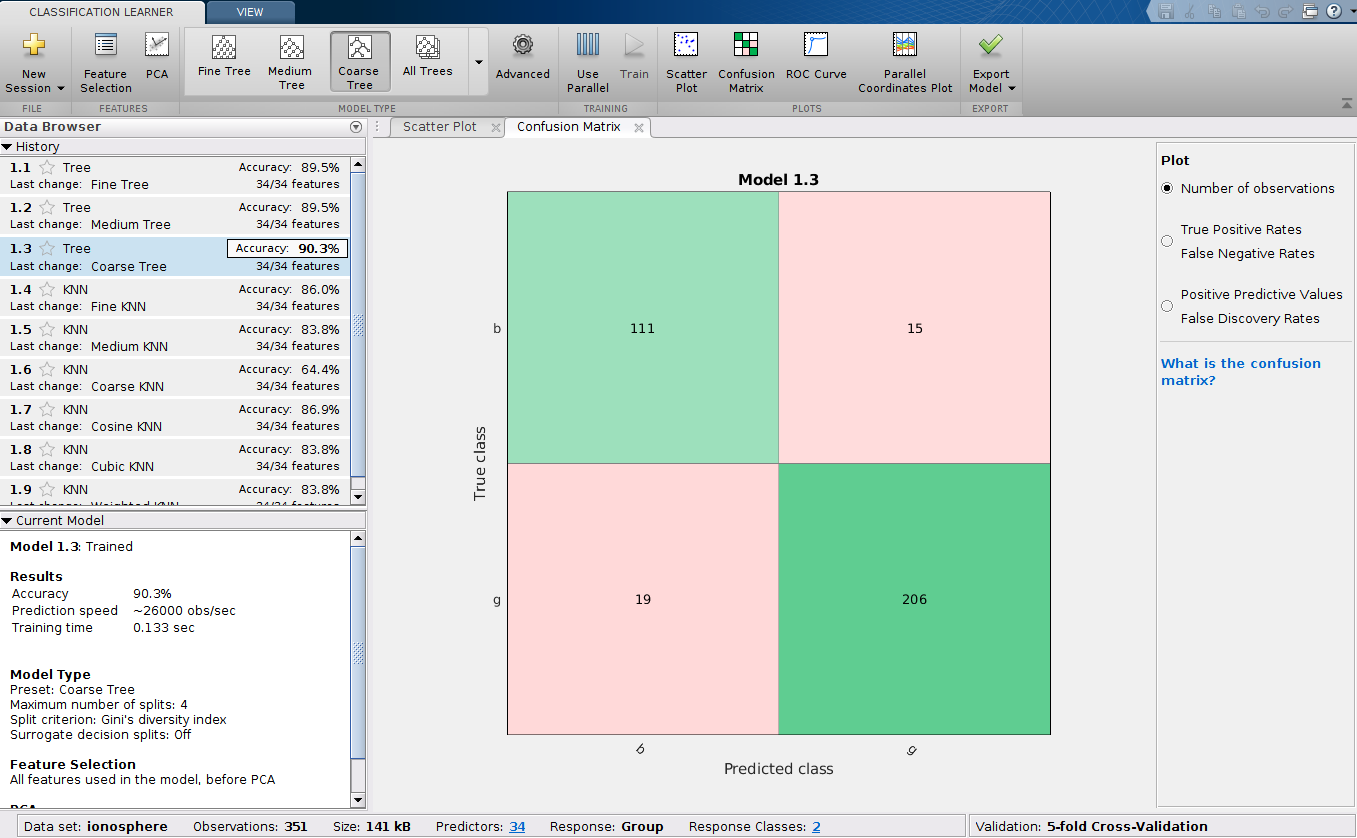
\includegraphics[width=\textwidth]{04-Methodology/mlClassificationLearner.png}
    \caption{Classification example in Matlab}
    \label{fig:classLearnerSamp}
\end{figure}
Matlab is a tool widely used for the numerical analysis of data and offers a wide range of additional add-ons, a large community backing, and an efficient backend. One of the add-ons available in Matlab is the \emph{Classification Learner}. This is a tool that takes a dataset as input, requests the specification of the features and classes in the dataset, and then quickly trains a number of different classifiers against the data, reporting the individual classifier accuracy, confusion matrix, and receiver-operating-characteristic (ROC) curve. This tool is therefore very useful for quickly getting an idea of how the different forms of classifier are dealing with the given features and classes. A diagram of the Classification Learner tool in use is shown in Figure \ref{fig:classLearnerSamp}. Here the comparison between the classifiers can be seen, along with the confusion matrix for one of the classifiers.\\

\begin{figure}[ht]
    \centering
    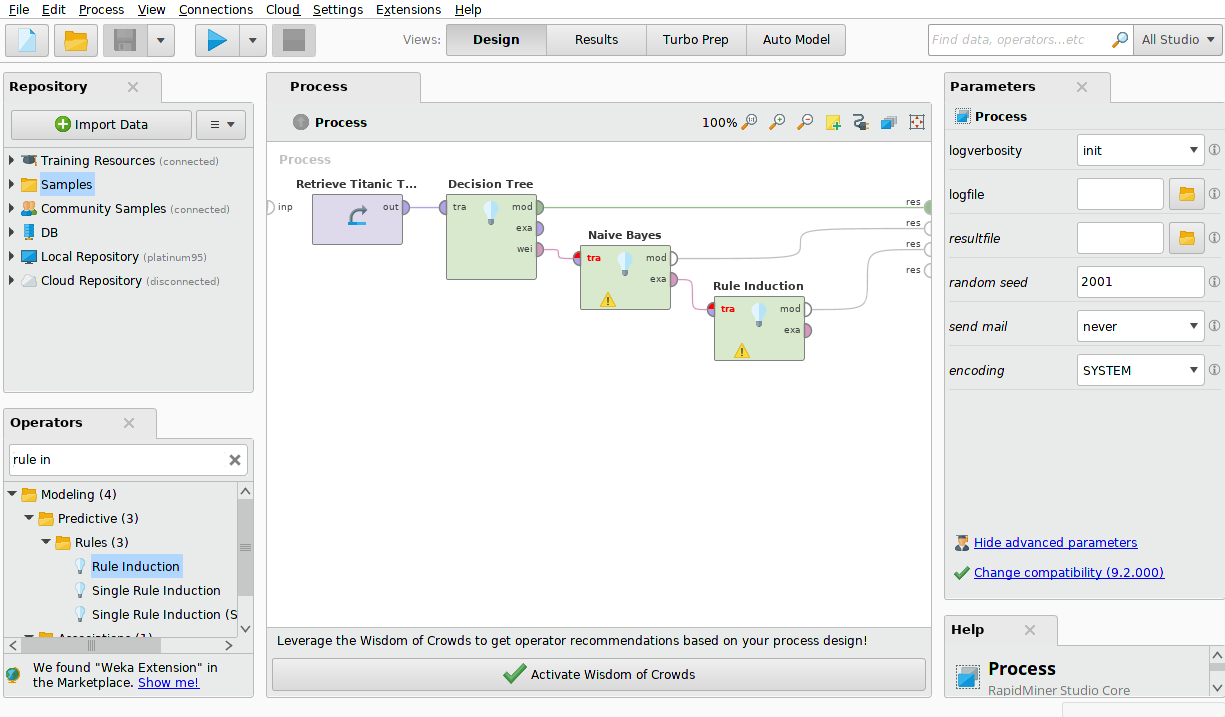
\includegraphics[width=\textwidth]{04-Methodology/rapidMinerUI.png}
    \caption{Classification example in RapidMiner}
    \label{fig:rapidMinerUi}
\end{figure}
For more fine-grained control of the classifier parameters, RapidMiner was used. RapidMiner is a tool that is used in "Big Data" for the analysis of large sums of data. It features a node-link type graphical interface in which the user can construct data processing pipelines involving various stages of data passthrough, as well as a wide range of classification and machine-learning algorithms. A diagram of the user interface of RapidMiner with an example data-processing pipeline is shown in Figure \ref{fig:rapidMinerUi}.\\

%TODO: Fill out this section with the specific layout of the rapidminer pipeline used for classifying.

\subsection{Cell-Type Segregation}
% TODO: Discussion of the splitting of a given cell into associated layer, m-type, and e-type to make classification easier.\\
% Discussion of the classifier stacks (i.e. output of layer-classifier as input to m-type classifier etc) and why this was done (layer/m-type/e-type not mutually independent).
We have previously discussed how each of the cells in the dataset has been classified by the BBP; that is, each cell has an associated layer, m-type, and e-type. As there are over 1000 individual cell models, it is unlikely that a classifier will be capable of gaining any form of functional accuracy in directly classifying the exact cell type. For this reason, the classification of a given cell was broken down in the classification of each of its constituent components, i.e. 3 separate classifiers were trained to estimate the cell type. The first classifier estimates the layer to which the cell belongs based on the filter coefficients extracted through equation \ref{eq:estFilter}. The second classifier estimates e-type based on the filter coefficients as well as the output of the first classifier (the layer estimation). The final classifier estimates m-type based on the filter coefficients, the estimated layer, and the estimated e-type. In this format, each classifier is only estimated against 5, 11, and 24 classes respectively. The other benefit of this approach is that the output of one classifier can be fed into the next, which allows the classifier to take into account the associated probability of one class leading to another, for example it might be more likely that layer 1 neurons contain more pyramidal m-types.\\
For training the classifiers, therefore, the "simulated cell" class will be broken down based on the cell identifier string. By splitting the string at all underscore characters ("\_") we can reliably extract the three constituent classes. For example, taking the cell identified by "L1\_DAC\_bNAC", splitting the string at all underscores results in three substrings, \{"L1", "DAC", "bNAC"\}, which correspond to the classes \{layer, m-type, e-type\}.

\subsection{Network Topographies and Tomography}
%Types of networks analysed (2-cell to train, 4-leaf to test tomography).
%Discussion on the tomography of the reconstruction of the cell-types, i.e. applying the pre-trained models to the 4-leaf network to estimate the cell-type of the leaves.
There are two main topologies investigated in this study: 2-cell topology, and 4-leaf star topology.
\par
\begin{wrapfigure}{R}{0.3\textwidth}
    \begin{center}
        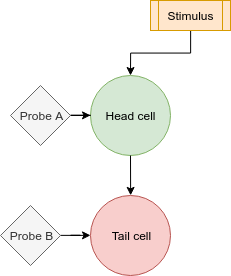
\includegraphics[width=0.3\textwidth]{04-Methodology/2cellTop.png}
    \end{center}
    \caption{2-cell Topology}
    \label{fig:2cellTop}
\end{wrapfigure}
The 2-cell topology is shown in Figure \ref{fig:2cellTop}. This 2-cell topology is quite simple as it is used mainly to analyse the link between two neurons rather than to study the various effects of neuronal layout. It consists of two cells linked by a synaptic connection whose parameters vary between network to network. A probe is attached to each cell to measure the output spike trains at all times in the simulation. A stimulus is also connected to the "head" node, whose parameters also vary between simulation to simulation.

\par


The 4-leaf star topology is shown in Figure \ref{fig:4leafStar}. This is a slightly more complex network than the 2-cell topology. The intention of the use of this network is to analyse the application of the results found from the study of the 2-cell networks in more complex topologies to investigate what effects, if any, the topology may have on performance. It is important to note here that the direction of the synaptic connections is that of an "out-hub", i.e. the central node (acting as the hub) is delivering voltage spikes to the surrounding leaves. This is in contrast to the 4-leaf star layout previously analysed \cite{ekkyProj} where the 4-leaf star topology acted as an "in-hub" with the leaf nodes delivering spike-events to the central node.
\begin{figure}[ht]
    \centering
    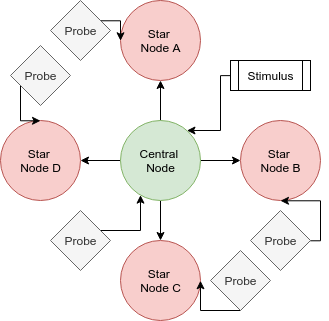
\includegraphics[width=0.5\textwidth]{04-Methodology/4cellTop.png}
    \caption{4-leaf star Topology}
    \label{fig:4leafStar}
\end{figure}
\par

For the investigation of the neuronal classification, the topologies will be used in the following manner. The voltage measurements taken from the database of 2-cell networks will be used to train the classification models, and to compare the performance difference between the different algorithms. When the classification models have been fully trained, they will be applied on the voltage measurements of the 4-leaf star topology simulations. The classifier will then attempt to estimate the type of cell used in each leaf node in order to reconstruct the topology; in other words, the classifier will be used to apply network tomography to estimate the parameters of the 4-leaf star network from a number of endpoint measurements. The performance of the classifier in this application will be compared against the performance in the 2-cell networks and differences will be discussed (if any).
